% !TeX program = pdfLaTeX
\documentclass[12pt]{article}
\usepackage{amsmath}
\usepackage{graphicx,psfrag,epsf}
\usepackage{enumerate}
\usepackage{natbib}
\usepackage{textcomp}
\usepackage[hyphens]{url} % not crucial - just used below for the URL
\usepackage{hyperref}
\providecommand{\tightlist}{%
  \setlength{\itemsep}{0pt}\setlength{\parskip}{0pt}}

%\pdfminorversion=4
% NOTE: To produce blinded version, replace "0" with "1" below.
\newcommand{\blind}{0}

% DON'T change margins - should be 1 inch all around.
\addtolength{\oddsidemargin}{-.5in}%
\addtolength{\evensidemargin}{-.5in}%
\addtolength{\textwidth}{1in}%
\addtolength{\textheight}{1.3in}%
\addtolength{\topmargin}{-.8in}%

%% load any required packages here



% Pandoc citation processing


\begin{document}


\def\spacingset#1{\renewcommand{\baselinestretch}%
{#1}\small\normalsize} \spacingset{1}


%%%%%%%%%%%%%%%%%%%%%%%%%%%%%%%%%%%%%%%%%%%%%%%%%%%%%%%%%%%%%%%%%%%%%%%%%%%%%%

\if0\blind
{
  \title{\bf An Examination of Sport Climbing Competition Format and
Scoring System}

  \author{
        Author 1 \thanks{Corresponding author: Name. Email:} \\
    \\
     and \\     Author 2 \\
    \\
     and \\     Author 3 \\
    \\
      }
  \maketitle
} \fi

\if1\blind
{
  \bigskip
  \bigskip
  \bigskip
  \begin{center}
    {\LARGE\bf An Examination of Sport Climbing Competition Format and
Scoring System}
  \end{center}
  \medskip
} \fi

\bigskip
\begin{abstract}
The purpose of this paper is to investigate sport climbing, one of the
sports making its debut on the Olympics stage at Tokyo 2020. In
particular, we take a closer look at the controversial competition
format and scoring system of sport climbing\ldots{} Simulation. Data
Analysis: drop and re-rank, correlations
\end{abstract}

\noindent%
{\it Keywords:} sport climbing, scoring system, 2020 Summer Olympics
\vfill

\newpage
\spacingset{1.45} % DON'T change the spacing!

\hypertarget{introduction}{%
\section{Introduction}\label{introduction}}

In 2016, the International Olympic Committee announced the addition of
five new sports to the 2020 Summer Olympics in Tokyo, Japan, which would
then reschedule for 2021 due to the impact of the COVID-19 global
pandemic. The five new features to Tokyo 2020's competitions program
include baseball/softball, karate, skateboard, sports climbing, and
surfing. One of the new sports, sport climbing, got our attention,
specifically because of its unique scoring system and the fact that only
one set of medals is awarded for each gender.

Sport climbing at the 2020 Tokyo Olympics consists of three disciplines:
speed climbing, bouldering, and lead climbing. Speed climbing takes
place on a standardized course and competitors try to reach the top of
the course as fast as possible. For Tokyo 2020, speed climbing is being
contested in a head-to-head format with ranks determined by how far a
competitor advances in the bracket. In bouldering, contestants have a
fixed amount of time to complete as many courses as they can. Winners
are determined based on who completes the most courses and ties are
broken based on who had the fewest attempts. Ties are further broken by
the competitor achieved the most ``zone holds'', which are holds
approximately halfway through each course. Finally, in lead climbing, an
athlete gets one point for each hold that they reach, so whoever reaches
the highest point on the wall is the winner. Each lead climber only gets
one attempt and when they fall their attempt is over. These three
different climbing disciplines demand different sets of skills and,
often, athletes specialize in a single event. However, since only one
set of Olympic medals is awarded to sport climbing, rather than choosing
only one of these disciplines to include in the Olympics, all three
events were chosen to be included as a sort of climbing triathlon.

At the 2020 Summer Olympics, both men's and women's sport climbing
competitions begin with 20 climbers who has previously qualified for the
Olympics from qualifying events held in 2019 and 2020. All 20 athletes
compete in each of the three disciplines in the qualification round, and
their performances in each concentration are ranked from 1 to 20. A
competitor's total score is then computed as the product of their ranks
in the three events and the lower product is better; specifically,
\begin{equation}
Score_i = R^S_i\times R^B_i\times R^L_i,
\end{equation} where \(R^S_i\), \(R^B_i\), and \(R^L_i\) are the ranks
of the \(i\)-th competitor in speed climbing, bouldering, and lead
climbing, respectively.

The top 8 finishers in the qualification round advance to the finals
where they once again compete in all three of speed climbing,
bouldering, and lead climbing. The total score for each climber in the
final stage is determined by multiplying their ranks in each discipline,
similar to the qualification round. This implies that the climber with
the lowest product of ranks in the final wins the gold medal. This type
of scoring system heavily rewards high finishes and relatively ignores
poor finishes. For instance, if climber A finished 1st, 20th, and 20th
and climber B finished 10th, 10th, and 10th, climber B would have a
score of 1000 whereas climber A would have a much better score of 400,
despite finishing last in 2 out of 3 of the events.

Heavily criticized

Other sports scoring methods

The manuscript is outlined as follows. We first begin with some
descriptions of the data and methods in Section 2. Our analyses and
results are then presented in Sections 3 and 4. Finally, in Section 5,
we summarize up of main findings and give a discussion to close out the
paper.

\hypertarget{data-and-methods}{%
\section{Data and Methods}\label{data-and-methods}}

The first sets of data that we rely on are historical results from major
climbing competitions in the past. We collected data on climbing
contests that took place between 2018 and 2020, where the combined
format was used to determine the scores and ranks of climbers. The
events include the 2020 Continental Championships of Europe, Africa,
Oceania, Pan-America; 2019 and 2018 World Championships; 2018 Asian
Games; and 2018 Youth Olympics. Data were obtained from various sources,
including the event websites, Wikipedia, and the International
Federation of Sport Climbing (IFSC). The main attributes of our datasets
are the name and nationality of the climbers; bib number (for some
competitions); the finishing place of climbers in speed climbing,
bouldering, and lead climbing; the total score (which equals the product
of event ranks); and the final rank. We utilize this data to compute the
correlations between the event ranks and final table position, as well
as to look at how often the final orderings change if one athlete is
dropped and the ranks for each discipline are re-computed.

Our second data source comes from a simulation study that we conducted,
with the purpose of examining the rankings and scoring for climbers in
both qualification and final rounds. For each round, we performed 10000
simulations, and this was accomplished by randomly assigning the ranks
of each event to every participant, with the assumption that the ranks
are uniformly distributed. After the completion of the simulations, we
calculated the total scores for every simulated round, as well as the
final standings for the climbing athletes. The simulation results allow
to answer questions about various topics, including the distributions of
scores for qualifying and final rounds, and the probabilities of
advancing to the finals or winning a medal, given certain conditions.

Table 1 and Figure 1 are numerical and visual summaries of climbing
total score obtained from our simulated data for the qualification
round.

\begin{table}[ht]
\centering
\caption{Descriptive statistics of simulated scores for qualification and final rounds} 
\begin{tabular}{lrrrrrrrr}
  \hline
round & min & Q1 & median & Q3 & max & mean & sd & n \\ 
  \hline
Qualification & 1.00 & 240.00 & 684.00 & 1638.00 & 8000.00 & 1158.84 & 1273.48 & 200000 \\ 
  Final & 1.00 & 24.00 & 60.00 & 126.00 & 512.00 & 91.12 & 91.35 & 80000 \\ 
   \hline
\end{tabular}
\end{table}

\begin{figure}
\centering
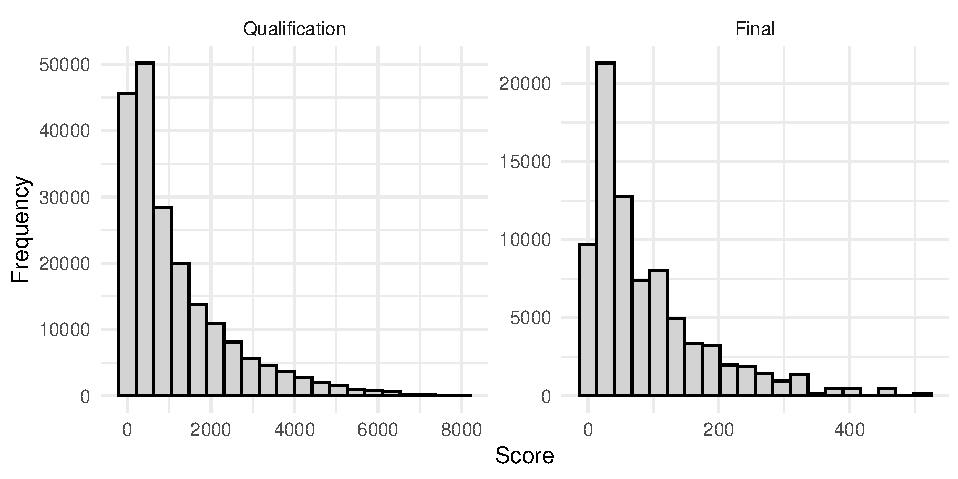
\includegraphics{draft_files/figure-latex/unnamed-chunk-5-1.pdf}
\caption{Histogram of simulated scores for qualification and final
rounds}
\end{figure}

\hypertarget{simulations}{%
\section{Simulations}\label{simulations}}

For the qualification round, a climber is almost guaranteed to make the
final round if they win the first event (with a 99.51\% chance of
advancing) or if they win at least one of the three climbing
concentrations (99.48\%). On the other hand, finishing last in the first
event or in any event would certainly hurt an athlete's chance of
finishing in the top 8, as the probabilities of a climber advancing
given they finish last in the first and in any event are 0.1830 and
0.1885, respectively. In addition, the average score for qualification
positions 1 to 8 are displayed in Table 1. We notice that on average,
the minimum score that one should aim for in order to move on to the
final round is 435 (for 8th rank).

\begin{table}[ht]
\centering
\caption{Average score for each qualifying rank} 
\begin{tabular}{rr}
  \hline
rank & avg\_adv\_score \\ 
  \hline
  1 & 36.02 \\ 
    2 & 73.61 \\ 
    3 & 115.40 \\ 
    4 & 162.23 \\ 
    5 & 216.00 \\ 
    6 & 278.16 \\ 
    7 & 350.33 \\ 
    8 & 434.59 \\ 
   \hline
\end{tabular}
\end{table}

Regarding the finals, a climber is very likely to earn a medal (finish
in the top 3) if they win the first event (83.03\% chance) or any event
(85.01\%). In order to obtain a climbing medal, the average score for
getting gold, silver, and bronze are 9.6748, 20.4143, and 33.2648,
respectively (Table 2).

\begin{table}[ht]
\centering
\caption{Average score of medalists} 
\begin{tabular}{rr}
  \hline
rank & avg\_score \\ 
  \hline
  1 & 9.67 \\ 
    2 & 20.41 \\ 
    3 & 33.26 \\ 
    4 & 50.59 \\ 
    5 & 74.76 \\ 
    6 & 110.05 \\ 
    7 & 164.43 \\ 
    8 & 265.78 \\ 
   \hline
\end{tabular}
\end{table}

\hypertarget{data-analysis}{%
\section{Data Analysis}\label{data-analysis}}

Corr

Drop 1

\hypertarget{speed-climbing-vs-lead-and-bouldering}{%
\subsection{Speed climbing vs lead and
bouldering}\label{speed-climbing-vs-lead-and-bouldering}}

For our analysis on the relationship between the rankings of the events
and the final result, we used data from the 2018 Youth Olympics Women's
Qualification. Figure 3 is a scatterplot and correlation matrix between
the ranks of the individual events and the final standings, with
Kendall's Tau (Kendall Rank Correlation Coefficient) as our measure of
ordinal association between the quantities. It is evidently clear that
there is a strong and positive correlation between the ranks of
bouldering and lead climbing, and as a results, the standings of these
two events are highly correlated with the final rankings. On the other
hand, the correlation with the final rank is not as strong for speed
climbing. Thus, speed climbers are facing a huge disadvantage in this
scoring system, compared to those that are specialized in the other two
concentrations.

This trend also holds for most of the past competitions.

\begin{figure}
\centering
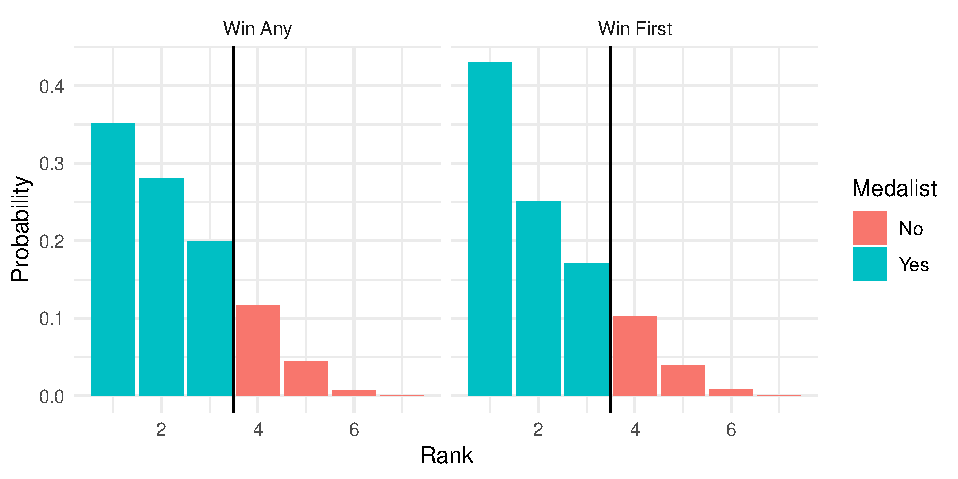
\includegraphics{draft_files/figure-latex/unnamed-chunk-10-1.pdf}
\caption{Kendall's rank correlations - 2018 World Championship, Women's
Qualification}
\end{figure}

\hypertarget{drop-and-re-rank}{%
\subsection{Drop and re-rank}\label{drop-and-re-rank}}

A single climber excluded changes things drastically, especially order
of medalists.

The cases where someone behind you drops out and your ranking changes.

Example from 2018 youth, women's final dropping ranks 3 and 5 change the
medalist order

\begin{figure}
\centering
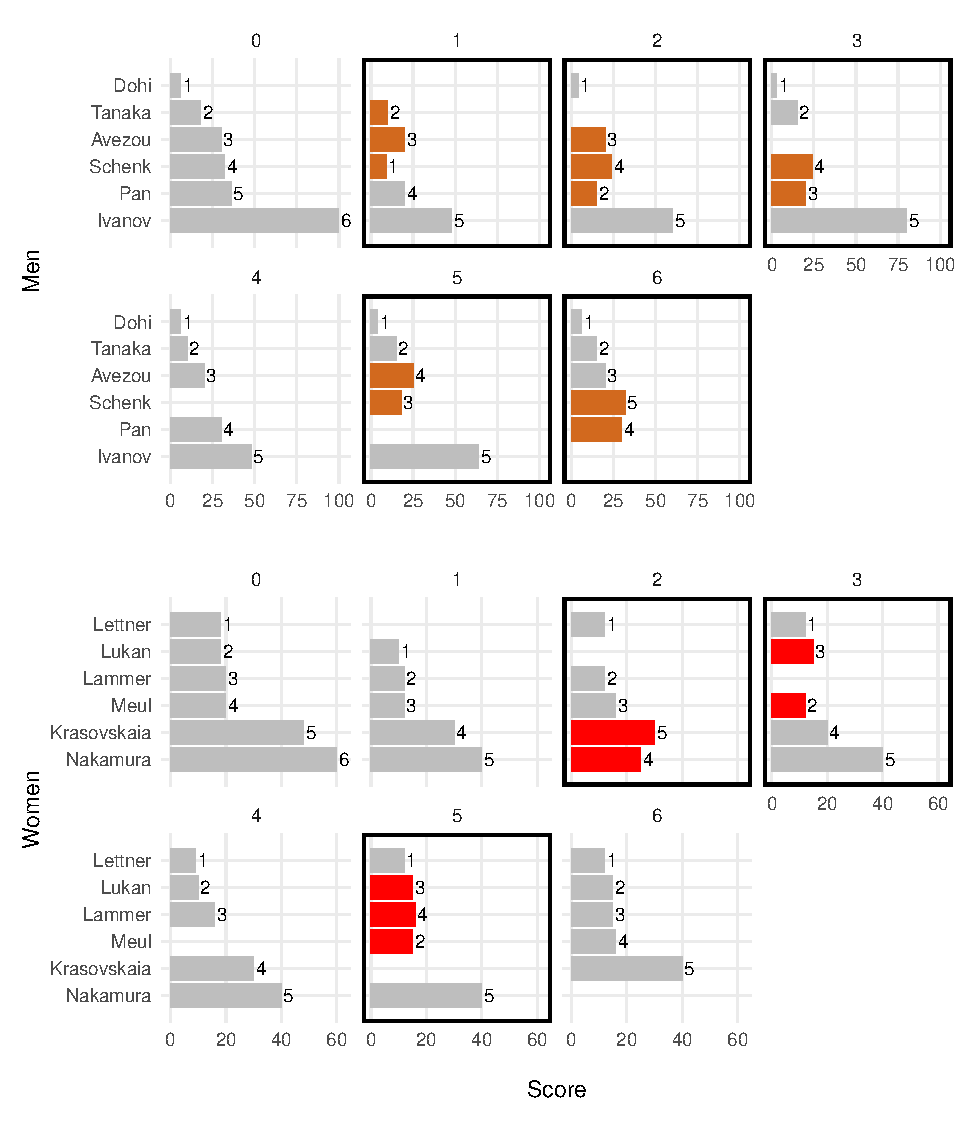
\includegraphics{draft_files/figure-latex/unnamed-chunk-12-1.pdf}
\caption{This figure shows the rankings of the Men's Sport Climbing
Final at the 2018 Youth Olympics. Each panel represents the dropped
rank, with 0 being the original final standings. The cases where a
change in ordering happened are highlighted.}
\end{figure}

\begin{figure}
\centering
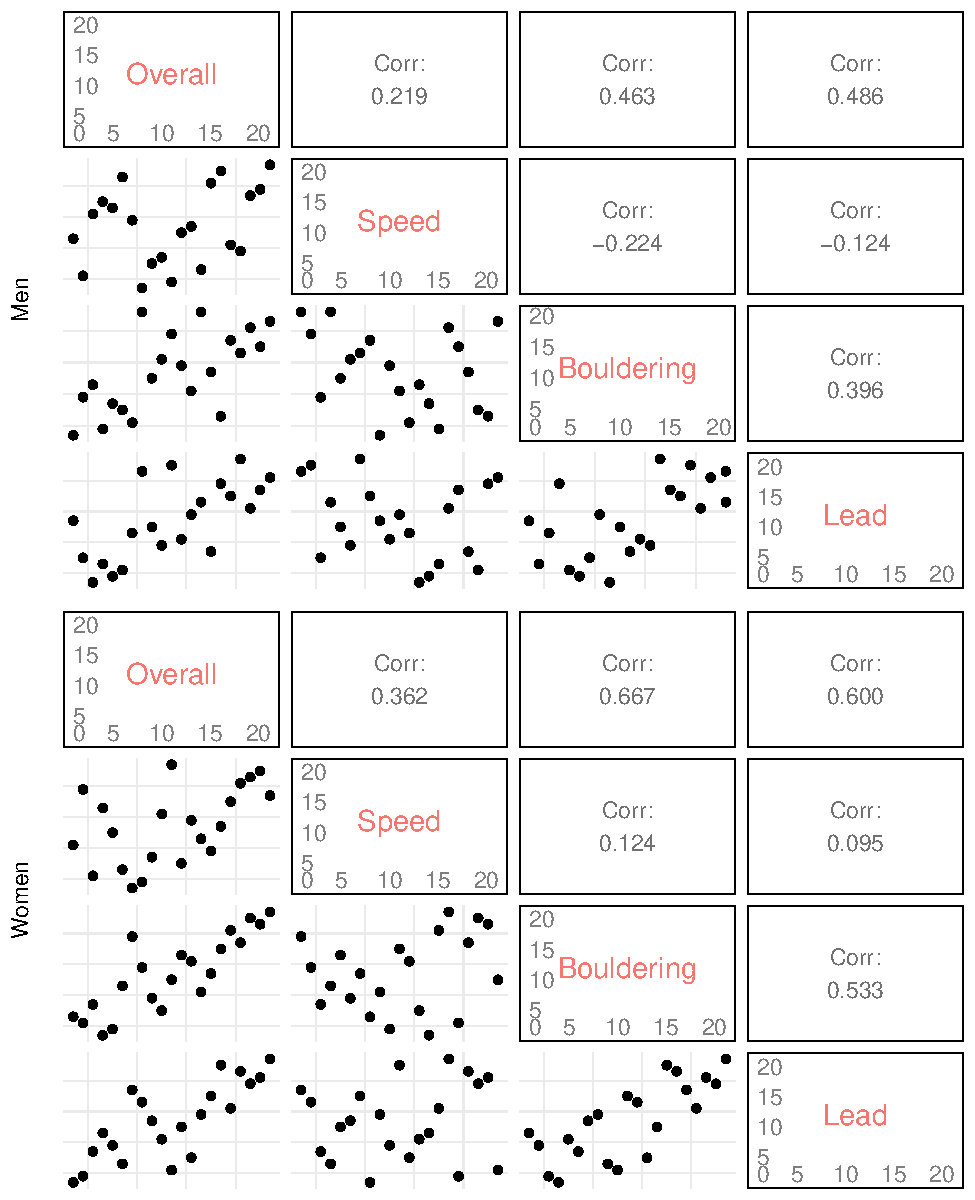
\includegraphics{draft_files/figure-latex/unnamed-chunk-13-1.pdf}
\caption{This figure shows the final rankings of 2018 Youth Olympics
Women's Final. Each panel represents the dropped rank, with 0 being the
original final standings. The cases where a change in ordering happened
are highlighted.}
\end{figure}

\bibliographystyle{agsm}
\bibliography{}

\end{document}
